%% BioMed_Central_Tex_Template_v1.06
%%                                      %
%  bmc_article.tex            ver: 1.06 %
%                                       %

%%IMPORTANT: do not delete the first line of this template
%%It must be present to enable the BMC Submission system to
%%recognise this template!!

%%%%%%%%%%%%%%%%%%%%%%%%%%%%%%%%%%%%%%%%%
%%                                     %%
%%  LaTeX template for BioMed Central  %%
%%     journal article submissions     %%
%%                                     %%
%%          <8 June 2012>              %%
%%                                     %%
%%                                     %%
%%%%%%%%%%%%%%%%%%%%%%%%%%%%%%%%%%%%%%%%%


%%%%%%%%%%%%%%%%%%%%%%%%%%%%%%%%%%%%%%%%%%%%%%%%%%%%%%%%%%%%%%%%%%%%%
%%                                                                 %%
%% For instructions on how to fill out this Tex template           %%
%% document please refer to Readme.html and the instructions for   %%
%% authors page on the biomed central website                      %%
%% http://www.biomedcentral.com/info/authors/                      %%
%%                                                                 %%
%% Please do not use \input{...} to include other tex files.       %%
%% Submit your LaTeX manuscript as one .tex document.              %%
%%                                                                 %%
%% All additional figures and files should be attached             %%
%% separately and not embedded in the \TeX\ document itself.       %%
%%                                                                 %%
%% BioMed Central currently use the MikTex distribution of         %%
%% TeX for Windows) of TeX and LaTeX.  This is available from      %%
%% http://www.miktex.org                                           %%
%%                                                                 %%
%%%%%%%%%%%%%%%%%%%%%%%%%%%%%%%%%%%%%%%%%%%%%%%%%%%%%%%%%%%%%%%%%%%%%

%%% additional documentclass options:
%  [doublespacing]
%  [linenumbers]   - put the line numbers on margins

%%% loading packages, author definitions

\documentclass[twocolumn]{bmcart}% uncomment this for twocolumn layout and comment line below
%\documentclass{bmcart}

%%% Load packages
%\usepackage{amsthm,amsmath}
%\RequirePackage{natbib}
%\RequirePackage{hyperref}
\usepackage[utf8]{inputenc} %unicode support
%\usepackage[applemac]{inputenc} %applemac support if unicode package fails
%\usepackage[latin1]{inputenc} %UNIX support if unicode package fails
\usepackage{amssymb}
\usepackage{graphicx}


%%%%%%%%%%%%%%%%%%%%%%%%%%%%%%%%%%%%%%%%%%%%%%%%%
%%                                             %%
%%  If you wish to display your graphics for   %%
%%  your own use using includegraphic or       %%
%%  includegraphics, then comment out the      %%
%%  following two lines of code.               %%
%%  NB: These line *must* be included when     %%
%%  submitting to BMC.                         %%
%%  All figure files must be submitted as      %%
%%  separate graphics through the BMC          %%
%%  submission process, not included in the    %%
%%  submitted article.                         %%
%%                                             %%
%%%%%%%%%%%%%%%%%%%%%%%%%%%%%%%%%%%%%%%%%%%%%%%%%


%\def\includegraphic{}
%\def\includegraphics{}



%%% Put your definitions there:
\startlocaldefs
\endlocaldefs


%%% Begin ...
\begin{document}

%%% Start of article front matter
\begin{frontmatter}

\begin{fmbox}
\dochead{Research}

%%%%%%%%%%%%%%%%%%%%%%%%%%%%%%%%%%%%%%%%%%%%%%
%%                                          %%
%% Enter the title of your article here     %%
%%                                          %%
%%%%%%%%%%%%%%%%%%%%%%%%%%%%%%%%%%%%%%%%%%%%%%

\title{Multifractal characterisation and classification of bread crumb digital images}

%%%%%%%%%%%%%%%%%%%%%%%%%%%%%%%%%%%%%%%%%%%%%%
%%                                          %%
%% Enter the authors here                   %%
%%                                          %%
%% Specify information, if available,       %%
%% in the form:                             %%
%%   <key>={<id1>,<id2>}                    %%
%%   <key>=                                 %%
%% Comment or delete the keys which are     %%
%% not used. Repeat \author command as much %%
%% as required.                             %%
%%                                          %%
%%%%%%%%%%%%%%%%%%%%%%%%%%%%%%%%%%%%%%%%%%%%%%

\author[
   addressref={aff1},                   % id's of addresses, e.g. {aff1,aff2}
   corref={aff1},                       % id of corresponding address, if any
   %noteref={n1},                        % id's of article notes, if any
   email={baravalle@cifasis-conicet.gov.ar}   % email address
]{\inits{RGB}\fnm{Rodrigo G} \snm{Baravalle}}
\author[
   addressref={aff2},
   email={cad@uns.edu.ar}
]{\inits{CAD}\fnm{Claudio A} \snm{Delrieux}}
\author[
   addressref={aff1},
   email={gomez@cifasis-conicet.gov.ar}
]{\inits{JCG}\fnm{Juan C} \snm{G\'omez}}

%%%%%%%%%%%%%%%%%%%%%%%%%%%%%%%%%%%%%%%%%%%%%%
%%                                          %%
%% Enter the authors' addresses here        %%
%%                                          %%
%% Repeat \address commands as much as      %%
%% required.                                %%
%%                                          %%
%%%%%%%%%%%%%%%%%%%%%%%%%%%%%%%%%%%%%%%%%%%%%%

\address[id=aff1]{%                           % unique id
  \orgname{Laboratory for System Dynamics and Signal Processing, FCEIA, Universidad Nacional de Rosario, CIFASIS-CONICET}, % university, etc
  \street{Ocampo y Esmeralda},                     %
  \postcode{S2000EZP}                                % post or zip code
  \city{Rosario},                              % city
  \cny{Argentina}                                    % country
}
\address[id=aff2]{%
  \orgname{Department of Electrical Engineering and Computers, Universidad Nacional del Sur - IIIE-CONICET},
  \street{Avenida Col\'on 80},
  \postcode{(8000FTN)}
  \city{Bah\'ia Blanca},
  \cny{Argentina}
}

%%%%%%%%%%%%%%%%%%%%%%%%%%%%%%%%%%%%%%%%%%%%%%
%%                                          %%
%% Enter short notes here                   %%
%%                                          %%
%% Short notes will be after addresses      %%
%% on first page.                           %%
%%                                          %%
%%%%%%%%%%%%%%%%%%%%%%%%%%%%%%%%%%%%%%%%%%%%%%

\begin{artnotes}
%\note{Sample of title note}     % note to the article
%\note[id=n1]{Equal contributor} % note, connected to author
\end{artnotes}

%\end{fmbox}% comment this for two column layout

%%%%%%%%%%%%%%%%%%%%%%%%%%%%%%%%%%%%%%%%%%%%%%
%%                                          %%
%% The Abstract begins here                 %%
%%                                          %%
%% Please refer to the Instructions for     %%
%% authors on http://www.biomedcentral.com  %%
%% and include the section headings         %%
%% accordingly for your article type.       %%
%%                                          %%
%%%%%%%%%%%%%%%%%%%%%%%%%%%%%%%%%%%%%%%%%%%%%%

\begin{abstractbox}

\begin{abstract} % abstract
Adequate models of the bread crumb structure can be critical for understanding flow and transport processes in bread manufacturing, creating synthetic bread crumb images for photo-realistic rendering, evaluating similarities, and establishing quality features of different bread crumb types.

In this article, multifractal analysis, employing the Multifractal Spectrum (MFS), has been applied to study the structure of the bread crumb in four varieties of bread ({\em baguette}, {\em sliced}, {\em bran}, and {\em sandwich}). The computed spectrum can be used to discriminate among bread crumbs from different types. Also, high correlations were found between some of these parameters and the porosity, coarseness, and heterogeneity of the samples. These results demonstrate that the MFS is an appropriate tool for characterising the internal structure of the bread crumb and thus it may be used to establish important quality properties it should have.

The MFS has shown to provide local and global image features that are both robust and low-dimensional, leading to feature vectors that capture essential information for classification tasks. Results show that the MFS based classification is able to distinguish different bread crumbs with very high accuracy. Multifractal modelling of the underlying structure can be an appropriate method for parameterising and simulating the appearance of different bread crumbs.


\end{abstract}

%%%%%%%%%%%%%%%%%%%%%%%%%%%%%%%%%%%%%%%%%%%%%%
%%                                          %%
%% The keywords begin here                  %%
%%                                          %%
%% Put each keyword in separate \kwd{}.     %%
%%                                          %%
%%%%%%%%%%%%%%%%%%%%%%%%%%%%%%%%%%%%%%%%%%%%%%

\begin{keyword}
\kwd{Fractal}
\kwd{Multifractal}
\kwd{Image analysis}
\kwd{Image classification}
\kwd{Feature extraction}
\end{keyword}

% MSC classifications codes, if any
%\begin{keyword}[class=AMS]
%\kwd[Primary ]{}
%\kwd{}
%\kwd[; secondary ]{}
%\end{keyword}

\end{abstractbox}
%
\end{fmbox}% uncomment this for twcolumn layout

\end{frontmatter}

%%%%%%%%%%%%%%%%%%%%%%%%%%%%%%%%%%%%%%%%%%%%%%
%%                                          %%
%% The Main Body begins here                %%
%%                                          %%
%% Please refer to the instructions for     %%
%% authors on:                              %%
%% http://www.biomedcentral.com/info/authors%%
%% and include the section headings         %%
%% accordingly for your article type.       %%
%%                                          %%
%% See the Results and Discussion section   %%
%% for details on how to create sub-sections%%
%%                                          %%
%% use \cite{...} to cite references        %%
%%  \cite{koon} and                         %%
%%  \cite{oreg,khar,zvai,xjon,schn,pond}    %%
%%  \nocite{smith,marg,hunn,advi,koha,mouse}%%
%%                                          %%
%%%%%%%%%%%%%%%%%%%%%%%%%%%%%%%%%%%%%%%%%%%%%%

%%%%%%%%%%%%%%%%%%%%%%%%% start of article main body
% <put your article body there>

%%%%%%%%%%%%%%%%
%% Background %%
%%
\section{Introduction}
\label{intro}
The goals of this research are: (1) to evaluate if the MFS \cite{Xu2009} can be applied to characterise and discriminate the bread crumb structure for different bread types from digital images, and (2) to investigate the effectiveness of the method in the classification of these structures.

One of the most important factors to evaluate the quality of a bread loaf is related to its crumb structure. Close examination of different slices reveals considerable variation in the cell (air bubble) size even within a single sample of the same bread type. 

Fractal and multifractal analysis of images have pro\-ved to be able to capture useful properties of the underlying material being represented. These features have been successfully applied in different areas, such as medi\-cine \cite{Andjelkovic2008,Yu2011} and texture classification \cite{Wendt2009}. In food research, fractal and multifractal analysis has been applied in the study of apple tissues \cite{Mendoza2010}, pork sirloins \cite{Serrano2012}, and also in chocolate, potato and pumpkin surfaces \cite{Quevedo2002}. Through several procedures \cite{Peitgen2004,Gonzales2008}, it is possible to obtain different Fractal Dimensions (FD), each of them capturing a different property of the material ({\em e.g.}, porosity, rugosity).

Data analysis of the results of the feature extraction process is useful for obtaining key properties of materials. This information could then be used in quality measurements of real samples and in the validation of synthetic representations of them. In other words, these processes are useful to determine if a given image presents the observed features in that material, allowing to associate quality measure parameters to it. In~\cite{Fan2006}, a bread crumb quality test based on Gabor filters was performed, obtaining good quality assessment. Nevertheless, a small database was used ($30$ images). In \cite{Gonzales2008} several fractal features were obtained for one type of bread, demonstrating that a vector of FDs would be capable of obtaining key features of the crumb texture more accurately than using a single FD.

In this work we propose the application of the Multifractal Spectrum (MFS) to describe and classify different bread crumb types. One of the main features of the MFS is its bi-Lipschitz invariance, that is, invariance to perspective transforms (viewpoint changes) and smooth texture surface deformations. It is shown that the MFS is also locally invariant to affine changes in illumination. In other words, MFS analysis is in theory a robust feature extractor, what makes it specially adequate for the purposes of our study.

Food classification has already been applied using fractal and other techniques in \cite{Zong2010,Bosch2011} but these works do not address the intra-class problem, {\em i.e.}, the classification is made among different foods and not by making different classes out of the same food.

In a previous work \cite{Baravalle2012_2}, we showed that the MFS in combination with other fractal features was able to classify different bread crumb types with high accuracy. The present work aims to simplify the model and strengthen these results by comparing {\em only} the MFS with other state-of-the-art features and using different classifiers, and also to study the correlations of the features obtained with the procedure and different texture features obtained from the images.

The proposed method is compared to other state-of-the-art features for texture classification. The results of this feature extraction procedure show that the classifier is robust and presents good discrimination properties to distinguish between different bread types and also bread from non bread images.

This paper is organised as follows. In section 2 the theory underlying fractal sets is introduced, and the materials and methods employed in this work are presented. In section 3 the results obtained in the characterisation and classification procedures are shown and discussed. In section 4 the conclusions are summarised, as well as possible future works.

\section{Materials and Methods}
\label{sec:1}
\subsection{Fractals and Multifractals}
\label{sec:2}

The term {\em fractal} was first employed by the mathematician B. Mandelbrot in \cite{Mandelbrot83}. Fractal objects have the property of self-similarity ({\em i.e.}, the geometrical or topological properties are invariant at different scales), and they are characterised by a non-integer dimension. Fractal objects can have one or more FDs. Most of the famous fractal sets ({\em i.e.}, the Cantor set, the Von Koch curve, and the Sierpinski gasket) can be characterised by a single exponent that relates how their geometrical properties vary under scale changes. On the other hand, there are cases where the fractal object exhibits different exponents under different scales. Those are called {\it multifractals} \cite{Mandelbrot89}, and are characterised by a sequence of FDs, or even a function that establishes the local variance of the geometrical properties under scale changes. It is assumed that these structures are composed by different fractals coexisting simultaneously. The self-similarity, then, can be characterised by a multifractal spectrum that establishes the specific fractal behaviour of the set at a given scale. The multifractal approach characterises better the objects than the fractal one, since variations in local regions are captured in a more accurate manner. A particular definition of dimension, the so-called Box Dimension, is employed in fractal and multifractal analysis.


\subsubsection{Box Dimension}
\label{sec:3}
On the one hand, mathematical objects such as the Koch curve and the Sierpinski triangle have exact self-similarity. Natural phenomena, on the other hand, are better described by statistical self-similarity. In such cases, the Box FD is used. Box FD is a simplification of the Hausdorff (originally Minkowski - Bouligand) dimension for non strictly self-similar objects \cite{Peitgen2004}. Given an image I, it is subdivided in a regular grid of boxes of side $\varepsilon$. If $N_{\varepsilon}$ represents the amount of boxes that contain at least one point of I for that $\varepsilon$, then the box dimension  $D_{b}$ is defined as

\begin{equation}
D_{b} \triangleq \displaystyle\lim_{\varepsilon \to 0}{\frac{\log(N_{\varepsilon})}{\log (1/\varepsilon)}}.
\label{eqn:1}
\end{equation}

A practical algorithm for computing $D_{b}$ in digital binarised images establishes different partitions of the original image in regular grids of side $\varepsilon$ (in pixels) and counts for each partition the amount $N_{\varepsilon}$ of boxes that contains at least one pixel of the object of interest. It uses a binarised image and selects different values of $\varepsilon$ in it, making a count of the boxes that contains pixels in each case. Since this procedure is not invariant under translations, an average of grid counting is performed under several translations at a given grid size $\varepsilon$. With the previous steps, a set of $\{1/\varepsilon, N_\varepsilon\}$ pairs is obtained, with which a linear fit is performed in log-space. Finally, the slope of the resulting straight line is by definition the box dimension of the image. In Fig.~\ref{fig:fitbox} an image of the bread type {\em bran} is shown (left), with an example of binarisation (centre) and its corresponding box dimension computation (right).


\subsection{The Theory behind Multifractal Analysis}
\label{sec:4}

In \cite{Gonzales2008}, several procedures were applied to analyse the bread crumb structure showing that a vector of FDs could better characterise those structures. Based on that assumption, in this work a multifractal analysis of the bread crumb is carried out. The idea behind multifractal analysis is to examine, in the limit, the local behaviour of a measure $\mu$ at each point of the set under study. 

Let $E$ be a structure divided in disjoint substructures $E_{i}$ of size $\varepsilon$ in such a way that 

\begin{equation}
\displaystyle\bigcup_{i}E_{i} = E.
\end{equation}

Each substructure $E_{i}$ is characterised by a measure $\mu(E_{i})$. From the point of view of multifractal analysis, it is useful to define the H\"older exponent, $\alpha_{i}$, for each substructure $E_{i}$, as a function of $\varepsilon$, {\em i.e.}


\begin{equation}
\alpha_{i} \triangleq \frac{ln(\mu(E_{i}))}{ln(\varepsilon)},
\label{eqn:eqn4}
\end{equation}
\noindent
and to take the limit when $\varepsilon$ tends to $0$. The limit $\alpha$ represents the value of the H\"older exponent at a point in the structure, that is

\begin{equation}
\alpha = \lim_{\varepsilon\to0}{\alpha_{i}}.
\label{eqn:eqn5}
\end{equation}

This exponent characterises the local regularity of the structure at a point. To obtain a global characterisation of the regularity of the structure it is necessary to obtain the distribution of $\alpha$ in $E$. Then, the multifractal spectrum related to the value of $\varepsilon$, $f_{\varepsilon}(\alpha_{i})$, is obtained by counting the $N_{\varepsilon}$ boxes characterised by $\alpha_{i}$, in the form:

\begin{equation}
f_{\varepsilon}(\alpha_{i}) = - \frac{ln(N_{\varepsilon}(\alpha_{i}))}{ln(\varepsilon)}.
\label{eqn:eqn6}
\end{equation}

When $\varepsilon$ tends to $0$, the limiting value is the FD of the structure $E$ characterised by $\alpha$ (the Hausdorff dimension of the $\alpha$ distribution). It is also known as the {\em multifractal spectrum} $f(\alpha)$ (MFS) \cite{Silvetti2010}, {\em i.e.}

\begin{equation}
f(\alpha) = \lim_{\varepsilon\to0}{f_{\varepsilon}(\alpha)}.
\label{eqn:eqn7}
\end{equation}

\subsubsection{Practical procedure for the MFS}
There are several techniques described in the literature to obtain the MFS, which lead to different representations of the multifractal information present in the structure. Usually, the method of moments is used \cite{Mendoza2010,Serrano2012}, but it produces a feature vector which is not always suitable for classification tasks. In this work, the procedure presented in \cite{Xu2009} is employed, due to its better classification performance.

The technique first computes $\alpha(x)$ for each pixel $x$ of the image. Denote with $B(x,\varepsilon)$ the closed disk of radius $\varepsilon > 0$ centred at $x$, then, $\alpha(x)$ is defined as a straight line fit of the values $log(\mu(B(x,\varepsilon)))$ and $log(\varepsilon)$. Then, a discrete sample set $\{\alpha_{i}, i = 1,\dots,M\}$ is taken from the interval $[0,1]$, and the point set corresponding to that value of $\alpha_{i}$ is formed by grouping the pixels with values that are close to that $\alpha_{i}$ under some threshold. The FD for each point set is computed as the straight line fit of the values $log((N_{\varepsilon}(\alpha_{i}))$ and $log(\varepsilon)$. The value M determines the vector length, {\em i.e.}. the number of FDs of the MFS.


As previously stated, the $f(\alpha)$ spectrum (MFS) and the method of moments produce vectors which contains the same information, but in this work the first is employed, since it also outperforms the method of moments in classification tasks. This process produces a finite vector which is used as the feature vector later in this paper. In next sections, the vector length (the number of FDs) is chosen based on the classification performance of the computed feature vector.


\subsubsection{Multifractal Measures}
Defining different $\mu$ functions accounts for different image features. The first approach is to define $\mu$ in the intensity domain (I), {\em i.e.}

\begin{equation}
\mu(B(x,\varepsilon)) = \int_{B(x,\varepsilon)}{(G_{\varepsilon} \ast I)} dx,
\label{eqn:eqn11}
\end{equation}
where $\ast$ is the $2D$ convolution operator and $G_{\varepsilon}$ is a Gaussian smoothing kernel with variance $\varepsilon$, {\em i.e., } $\mu$ is the weighted average intensity value in the disk of radius $\varepsilon$ centred at $x$ ($B(x,\varepsilon)$). This is the density of the intensity function, and it describes how the intensity at a point changes over scale.

The definition of $\mu$ could serve to specific purposes. For instance, if robustness to illumination changes is needed, one choice is to define $\mu(B(x,\varepsilon))$ on the domain of the energy of the gradients. Let ${ f_{k} , k = 1, 2, 3, 4}$ be four directional differential operators along (respectively) the vertical, horizontal, diagonal and anti-dia\-gonal directions. Then we define a measure function $\mu(B(x,\varepsilon))$ for the image $I$ as follows:

\begin{equation}
\mu(B(x,\varepsilon)) = (\int_{B(x,\varepsilon)}{\sum_{k}{(f_{k} \ast (G_{\varepsilon} \ast I))^{2}} dx)^{1/2}}.
\label{eqn:gradient}
\end{equation}

Another choice is to define $\mu(B(x, \varepsilon))$ as the sum of the Laplacians of the image inside $B(x, \varepsilon)$, that is

\begin{equation}
\mu(B(x,\varepsilon)) = \int_{B(x,\varepsilon)}|\nabla^2 (G_{\varepsilon} \ast I)| dx.
\label{eqn:laplacian}
\end{equation}

All these alternative measures modify the computed FD and MFS (except for trivial or monofractal images), and therefore are valuable choices in finding adequate features, as will be shown below.

\subsection{Image Acquisition}
\label{sec:7}
For testing our characterisation and classification procedures, $20$ images of $4$ different commercial bread types ({\em baguette}, {\em sliced}, {\em bran} and {\em sandwich}), counting $80$ images, were obtained in the same day of purchase using an HP PSC 1210 scanner with the following settings: highlight $190$, shadows $40$, and midtones $1$, and they were saved in TIFF format. Images were acquired at a resolution of $380 \times 380$ pixels (the maximum possible area for the four bread types) and $350$ dpi ($1$ pixel $= 0.00527$ $[mm^{2}]$). Then the images were converted to grey scale ($8$ bits). In addition, $20$ other images of each bread type were acquired with a digital camera, using the same spatial resolution. The illumination conditions of these images were different from that of the scanner in order to test for the robustness of the method. In Fig.~\ref{fig:camera} four examples of bread images obtained with the camera are shown. We also employed $100$ randomly selected images from the CalTech101 dataset~\cite{FeiFei04} in order to test the method's performance with non-bread images.

The void fraction (VF), mean cell area (MCA) and standard deviation of mean cell area (stCA), were computed in order to study the relationship of the MFS with the porosity, coarseness and heterogeneity of the different bread crumbs. For this purpose, the scanned images (in grey scale) were binarised using the algorithm presented in \cite{White83}. This algorithm applies a local thresholding scheme, which showed better results than using a global thresholding scheme. Particularly, the algorithm presented in \cite{Huang95} and used in \cite{Gonzales2008}, showed poor results when the illumination conditions vary in the image. In Fig.~\ref{fig:bread} an image of each bread type used in this work (top row) and its resulting binarisation using the proposed algorithm (bottom row) are shown. Small elements of $1$ and $2$ pixels were eliminated by an opening operation (erosion and dilation) using a $2\times2$ structuring element. The method showed good results even for different illumination conditions varying in the same image. 

In order to determine the result of the binarisation at a given pixel, the algorithm obtains an average from the grey levels in a window surrounding the pixel, and compares it to a threshold determined by the actual grey level of the pixel multiplied by a bias factor, {\em i.e.}

\begin{equation}
\frac{\sum_{x,y \in W} f(x,y) }{W_{size}} \geq f(x_{c},y_{c}) \times bias,
\label{eqn:white}
\end{equation}
where $x_{c},y_{c}$ are the coordinates of the actual pixel, and $W$ is the window surrounding that pixel. Two parameters must be set in the algorithm: the size of the window ($W_{size}$) and the $bias$. It was found that different values for the bias are needed for better results when different capturing methods are used. The optimal values for the scanner samples were $80$ for the window size and $1.15$ for the bias. In the case of the digital camera samples, the optimal values found were $80$ for the window size and $1$ for the bias. These differences seem to be caused by the different illumination conditions present in the images resulting from these different capturing conditions. Further research is required in order to determine automatic values for these parameters.

\section{Results and discussion}
\label{sec:9}

In this section we will attempt to show how the MFS behave adequately as a feature descriptor able to distinguish bread from non-bread images. For this purpose, the MFS, using $20$ FDs, was computed for each of the $200$ images ({\em i.e.,} $40$ images of each bread type, and $40$ randomly selected nonbread images, getting $5$ balanced classes). In the next subsections we show how the computed data is analysed and used for classification purposes.


\subsection{Data Analysis}
\label{sec:11}

Self-organising maps (SOM)~\cite{Kohonen2001} of the feature vectors associated with each bread image were useful to represent them in a lower dimensional view, in order to better understand the meaning of their respective MFS. A SOM maps high dimensional data into a (typically) two-dimensional representation, using neighbourhood information. Topological information of the original data is preserved.

Unsupervised SOM of the multifractal representation of bread and non-bread images are shown in Fig.~\ref{fig:somfractal} in a grid of $10\times10$ cells (the behaviour observed is similar for different grid sizes). In the left image, the $5$ classes ({\em e.g.}: {\em baguette}, {\em sliced}, {\em bran}, {\em sandwich} and {\em nonbread}) are shown, while in the right image, the {\em nonbread} class has been removed, and then the SOM was recomputed for the remaining $4$ classes, in order to highlight details among the MFS of the different bread types. The multifractal features SOM appears to show easily separable classes. It seems that a classifier could potentially obtain low classification errors using the multifractal features, since the numbers representing different classes are clearly separated to each other, {\em i.e.}, there are almost no cells with two or more different numbers in it. A classifier can define regions of space (group of cells) for each class.

In Fig. \ref{fig:boxplotsMFS}, boxplots of the four different bread types are shown with the medians of each FD (in red) joined by a dashed line. Each FD corresponds to a value of $\alpha_{i}$. In our experiments, the MFS vector has $20$ FDs (for reasons that will be explained in the classification section). From this plot, it could be pointed out that in the first half of the MFS (first $10$ FDs, $\alpha \in [0,0.53)$), the dispersion of the FDs is higher than in the second half of the spectrum (last $10$ FDs, $\alpha \in [0.53,1]$). The spectrum in the last FDs tends to have a shape that identifies better a particular type of image. Usually, the spectra of the same class and the same capturing method have, in this part of the spectrum, a shape that is useful to characterise the class. Nevertheless the capturing method and the illumination conditions of the image influences this shape, {\em i.e.} these two factors alters the MFS of the image. In other words, there is not a unique shape for each class of bread type.

For the sake of completeness, in Fig. \ref{fig:meansMFS}, the mean values and the standard deviations of the MFS for the four different bread types are shown. This image shows, similarly to the SOM maps, that the MFS could potentially characterise and classify the different bread crumb types, since the mean values are different for each class. The standard deviations are also consistent with the results found in the boxplots. 

The Spearman correlation coefficient ($\rho$) for the four bread types between the fractal dimensions and the void fraction, mean cell area and standard deviation of mean cell area (in $[mm^{2}]$) are shown in Figs. \ref{fig:corrVF}, \ref{fig:corrMCA} and \ref{fig:corrMCAstdev}, respectively, as a function of fractal dimension. In order to better describe the results, only the scanned samples were employed to analyse these correlations. $\rho$ is preferred over Pearson's $R$ coefficient since it does not require a linear dependence to exhibit strong correlations in the underlying data.

In Fig. \ref{fig:corrVF}, it becomes clear that the coefficients behave similarly for the first $5$ dimensions ($\alpha \in [0,0.23]$) in all the bread types, but differently for the FD around $5$ and above. It could be concluded that the first $5$ dimensions are highly correlated with the void fraction (porosity) of the scanned samples. This means that the first FDs increase when the void fraction increase. Other FDs also have a high (positive or negative) correlation, but it depends on the bread type which dimension is correlated.

From the plots of the correlation coefficients of the MCA and stCA, in Figs. \ref{fig:corrMCA} and \ref{fig:corrMCAstdev} respectively, it could also be pointed out that the MCA has a higher correlation than the stCA with the FDs of the MFS. It means that the coarseness of the bread crumb structure could be better characterised by the features than its heterogeneity, using the MFS. In addition, the last $5$ fractal dimensions of the spectra ($\alpha \in [0.79,1]$) are highly (inversely) correlated with the MCA of the scanned samples. This implies that the last FDs increase when the MCA decrease. The same observation could be mentioned for the stCA of the samples, but the correlations are lower. In both cases, the correlation coefficients of the {\em sandwich} class are the lower among the bread types.

To summarise, the dimensions of the MFS which corresponds to $\alpha \in [0,0.23]$ are useful to measure the porosity of the scanned samples. Also, coarseness and heterogeneity could be measured by the dimensions with $\alpha \in [0.79,1]$. As was suggested in a previous work \cite{Gonzales2008}, the bread crumb structure is better characterised by the use of a vector of fractal dimensions, since the three properties could be measured by the MFS, employing different sections of this feature vector.

\subsection{Bread Classification}
\label{sec:10}

In order to test for the discriminative capability of the method, a classification experiment is made. Five classes are defined, {\em viz.}, {\em baguette}, {\em sliced}, {\em bran}, {\em sandwich} and {\em non-bread}, assigning $40$ images to each class. A comparison is made between the MFS and state-of-the-art features in the computer vision literature. This classification scheme corresponds to an intra-class problem, which is harder to solve than an ordinary inter-class one. 

K-fold cross validation is applied to the entire set (with $K=4$), employing three different classifiers: Support Vector Machines (SVM), Random Forests (RF) \cite{Breiman2001}, and Nearest Neighbors (NN). Results show that the MFS presents good classification performance regardless of the classifier employed. The \textsf{libsvm} implementation \cite{Chang2011} was used for the SVM classifier (with RBF kernel). In the case of the RF ($100$ trees) and the NN ($1$ neighbour) classifiers, the \textsf{scikit-learn} python library was employed.

In Table \ref{tab:number}, the classification performance of the method is tested using different number of FDs. When $20$ FDs are used, an useful combination of performance and low-di\-men\-sio\-na\-li\-ty is achieved (it shows the best classification results for the RF and NN classifiers), so this number of FDs is used in the following computations. 

In Table \ref{tab:mfs}, several combinations of different MFS obtained from the images, and their classification performance are shown. The MFS used in the study were computed based on the density of the intensity (MFS in the table), the Laplacian of the intensity (L), and the gradient of the intensity (G) (see section Multifractal Measures). In addition, another test is made, using the CIELab \cite{Hunter58} colour space. The key advantage of this colour space is that it tends to reduce the dependency of the resulting image colour on the device used in the capture. The intensity of the images is transformed to the CIELab space, and the MFS of the three separated channels ({\em L}, {\em a}, and {\em b}) are combined together, obtaining a vector of $60$ FDs. This combination showed the best classification performance. It means that adding colour information in the $a$ and $b$ channels is useful for better classification of different types of bread crumbs, when different capturing devices are used (in this case, a scanner and a digital camera).

In Table \ref{tab:other}, state-of-the-art features (Haralick \cite{Haralick73}, Local Binary Pattern (Lbp) \cite{Ojala96} and SIFT \cite{Lowe2004} features) are computed for the images. The best classification performance is obtained using the SIFT features, but a feature vector of length 128 is required for every image, and, in addition, computational space and time is needed to build internal structures ({\em e.g.} a {\em codebook}). 

For better understanding the classification results, confusion matrices of the classification procedures could be plotted. As an example, the confusion matrix (from the cross validation) of the best results, {\em i.e.} the CIELab method, employing the SVM classifier, can be seen in Table \ref{tab:confusionmatrix}. In each column of the matrix, the output of the classifier for the $40$ images of each class is tested for correctness. The table shows that only in a few cases the classifier returns an incorrect result. For instance, among the $40$ images of {\em sliced}, only $2$ are  classified as images from other classes, specifically as {\em baguette} and {\em sandwich} (column with heading {\em sliced}). The others classes behave similarly. Differentiation between {\em bread} and {\em nonbread} images has no errors ({\em i.e.} no image of a bread class is classified as {\em nonbread} and vice versa). The $97.5\%$ of the database is correctly classified ($5$ misclassifications out of $200$).

The classification performance of the MFS for the bread crumb database is the highest a\-mong the algorithms studied. The MFS captures robust and useful information for classification in low dimensional features. These results also agree with results obtained in \cite{Bosch2011} for the classification of other food products.



\section{Conclusions}
\label{sec:11}
The visual appearance of different types of bread crumbs can be successfully characterised by the multifractal dimensions of their digital images. The FDs obtained from the MFS method whose $\alpha \in [0,0.23]$ provided a good measure of the bread crumb porosity, meaning that the higher these FDs, the higher the measure. In addition, the FDs whose $\alpha \in [0.79,1]$ are useful to measure coarseness and heterogeneity of bread crumb. The MFS contains useful data to characterise the three measures, combining the information in one feature vector.

The use of multifractal features in bread crumb texture classification showed excellent performance. The MFS de\-monstrated to be accurate enough to perform a classification of different bread types and also to discriminate non bread from bread images. The classification performance of the MFS for the bread crumb database outperforms other state-of-the-art techniques employed in the computer vision literature. The information present in the MFS of the $L$, $a$ and $b$ channels of the CIElab colour space obtained the best classification performance in all the developed tests. This result appears to be a consequence of the different capturing devices used in this work. Also, it was shown that the MFS is sensitive to changes in the illumination conditions during image acquisition.

The results found could also be applied to validate synthetic samples, in the sense that they should have similar features to the bread type they are trying to simulate. The features found with the MFS could be employed to tune bread crumb quality parameters.


%\section*{Content}
%Text and results for this section, as per the individual journal's instructions for authors. %\cite{koon,oreg,khar,zvai,xjon,schn,pond,smith,marg,hunn,advi,koha,mouse}

%\section*{Section title}
%Text for this section \ldots
%\subsection*{Sub-heading for section}
%Text for this sub-heading \ldots
%\subsubsection*{Sub-sub heading for section}
%Text for this sub-sub-heading \ldots
%\paragraph*{Sub-sub-sub heading for section}
%Text for this sub-sub-sub-heading \ldots
%In this section we examine the growth rate of the mean of $Z_0$, $Z_1$ and $Z_2$. In
%addition, we examine a common modelling assumption and note the
%importance of considering the tails of the extinction time $T_x$ in
%studies of escape dynamics.
%We will first consider the expected resistant population at $vT_x$ for
%some $v>0$, (and temporarily assume $\alpha=0$)
%
%\[
% E \bigl[Z_1(vT_x) \bigr]= E
%\biggl[\mu T_x\int_0^{v\wedge
%1}Z_0(uT_x)
%\exp \bigl(\lambda_1T_x(v-u) \bigr)\,du \biggr].
%\]
%
%If we assume that sensitive cells follow a deterministic decay
%$Z_0(t)=xe^{\lambda_0 t}$ and approximate their extinction time as
%$T_x\approx-\frac{1}{\lambda_0}\log x$, then we can heuristically
%estimate the expected value as
%
%\begin{eqnarray}\label{eqexpmuts}
%E\bigl[Z_1(vT_x)\bigr] &=& \frac{\mu}{r}\log x
%\int_0^{v\wedge1}x^{1-u}x^{({\lambda_1}/{r})(v-u)}\,du
%\nonumber\\
%&=& \frac{\mu}{r}x^{1-{\lambda_1}/{\lambda_0}v}\log x\int_0^{v\wedge
%1}x^{-u(1+{\lambda_1}/{r})}\,du
%\nonumber\\
%&=& \frac{\mu}{\lambda_1-\lambda_0}x^{1+{\lambda_1}/{r}v} \biggl(1-\exp \biggl[-(v\wedge1) \biggl(1+
%\frac{\lambda_1}{r}\biggr)\log x \biggr] \biggr).
%\end{eqnarray}
%
%Thus we observe that this expected value is finite for all $v>0$ (also see \cite{koon,khar,zvai,xjon,marg}).



%%%%%%%%%%%%%%%%%%%%%%%%%%%%%%%%%%%%%%%%%%%%%%
%%                                          %%
%% Backmatter begins here                   %%
%%                                          %%
%%%%%%%%%%%%%%%%%%%%%%%%%%%%%%%%%%%%%%%%%%%%%%

\begin{backmatter}

\section*{Competing interests}
  The authors declare that they have no competing interests.

%\section*{Author's contributions}
%    Text for this section \ldots

%\section*{Acknowledgements}
%  Text for this section \ldots
%%%%%%%%%%%%%%%%%%%%%%%%%%%%%%%%%%%%%%%%%%%%%%%%%%%%%%%%%%%%%
%%                  The Bibliography                       %%
%%                                                         %%
%%  Bmc_mathpys.bst  will be used to                       %%
%%  create a .BBL file for submission.                     %%
%%  After submission of the .TEX file,                     %%
%%  you will be prompted to submit your .BBL file.         %%
%%                                                         %%
%%                                                         %%
%%  Note that the displayed Bibliography will not          %%
%%  necessarily be rendered by Latex exactly as specified  %%
%%  in the online Instructions for Authors.                %%
%%                                                         %%
%%%%%%%%%%%%%%%%%%%%%%%%%%%%%%%%%%%%%%%%%%%%%%%%%%%%%%%%%%%%%

% if your bibliography is in bibtex format, use those commands:
\bibliographystyle{bmc-mathphys} % Style BST file
\bibliography{bibliography}      % Bibliography file (usually '*.bib' )

% or include bibliography directly:
% \begin{thebibliography}
% \bibitem{b1}
% \end{thebibliography}

%%%%%%%%%%%%%%%%%%%%%%%%%%%%%%%%%%%
%%                               %%
%% Figures                       %%
%%                               %%
%% NB: this is for captions and  %%
%% Titles. All graphics must be  %%
%% submitted separately and NOT  %%
%% included in the Tex document  %%
%%                               %%
%%%%%%%%%%%%%%%%%%%%%%%%%%%%%%%%%%%

%%
%% Do not use \listoffigures as most will included as separate files

\section*{Figures}
\begin{figure*}[h!]
\centering
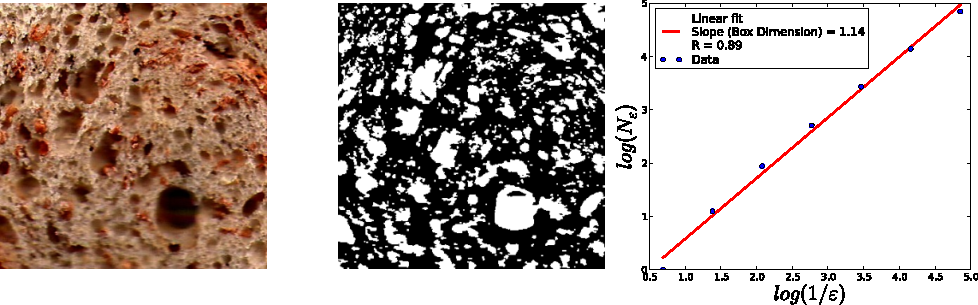
\includegraphics{Fig1}
\caption{\csentence{Box dimension computation.}
A bread image (left) with its binarisation (centre) and its computed box dimension (right).}
\label{fig:fitbox}
\end{figure*}

\begin{figure*}[h!]
\centering
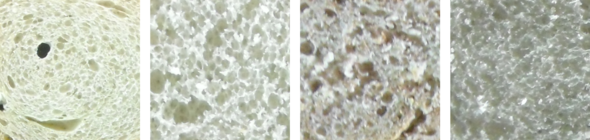
\includegraphics{Fig2}
\caption{\csentence{Images from a digital camera.}}
\label{fig:camera}
\end{figure*}

\begin{figure*}[h!]
\centering
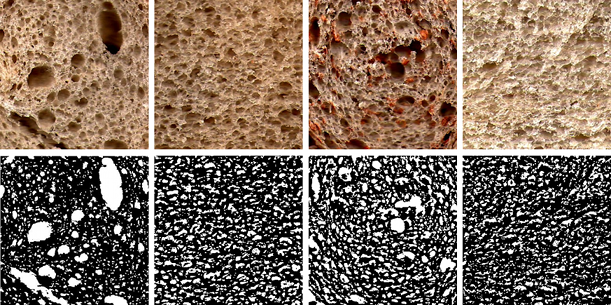
\includegraphics{Fig3}
\caption{\csentence{Images from a scanner.} {\em Baguette}, {\em sliced}, {\em bran} and {\em sandwich} bread types (top row) with their corresponding binarisations (bottom row).}
\label{fig:bread}
\end{figure*}

\begin{figure*}[h!]
\begin{centering}
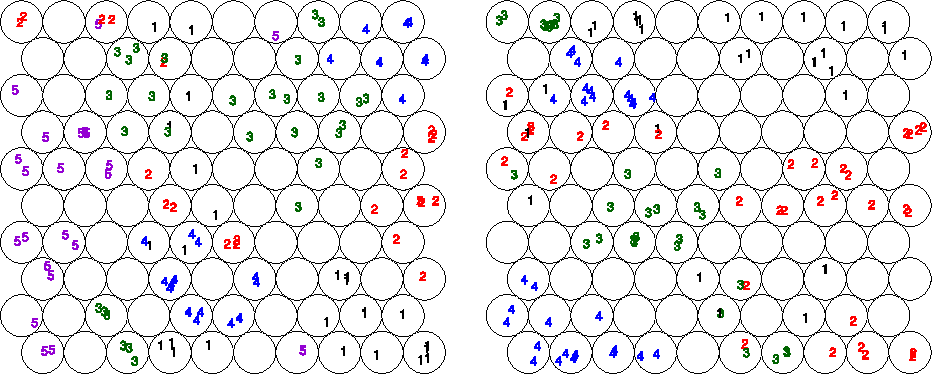
\includegraphics{Fig4}
\caption{\csentence{Self-organising maps (SOM).} SOM of the bread and non-bread images (left) and SOM of the bread types only (right). $1$: {\em baguette}, $2$: {\em sliced}, $3$: {\em bran}, $4$: {\em sandwich}, $5$: {\em nonbread}.}
\label{fig:somfractal}
\end{centering}
\end{figure*}

\begin{figure*}[h!]
\centering
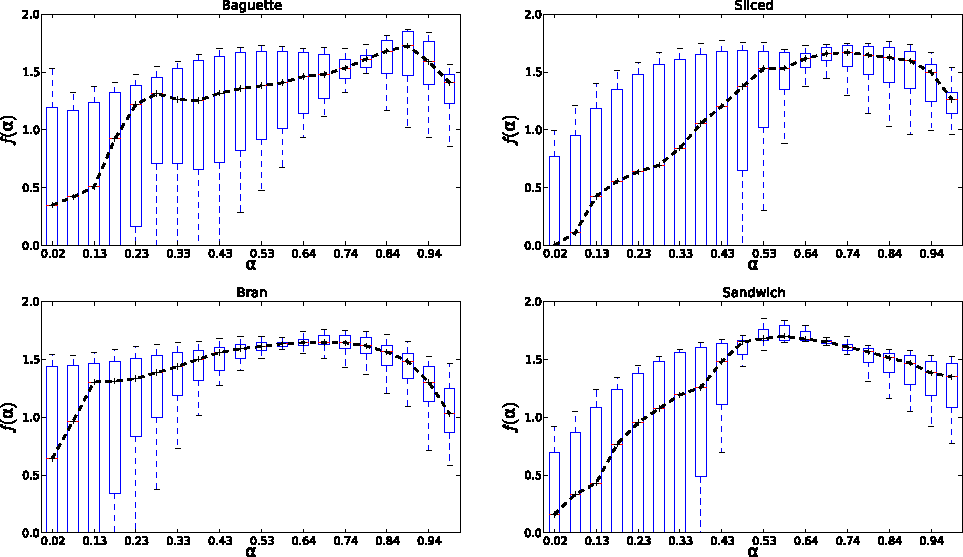
\includegraphics{Fig5}
\caption{\csentence{Boxplots of the four different bread types.} The FD medians are joined by a dashed line. Top: {\em baguette} (left), {\em sliced} (right), bottom: {\em bran} (left), {\em sandwich} (right).}
\label{fig:boxplotsMFS}
\end{figure*}

\begin{figure*}[h!]
\centering
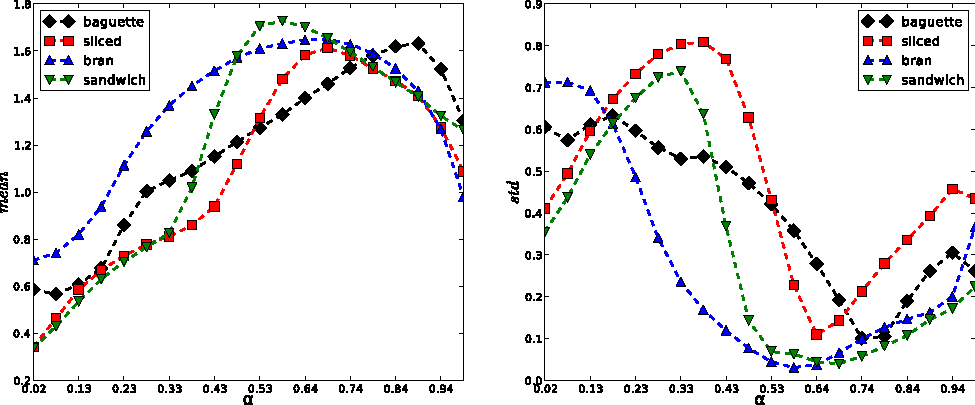
\includegraphics{Fig6}
\caption{\csentence{Mean MFS and standard deviations of the FDs for the four different bread types.} Left: mean MFS, right: standard deviations.}
\label{fig:meansMFS}
\end{figure*}


\begin{figure*}[h!]
\centering
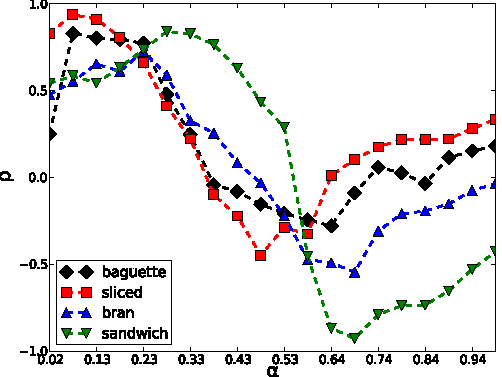
\includegraphics{Fig7}
\caption{\csentence{Spearman correlation coefficients for the FDs and the void fraction of the scanned samples.}}
\label{fig:corrVF}
\end{figure*}

\begin{figure*}[h!]
\centering
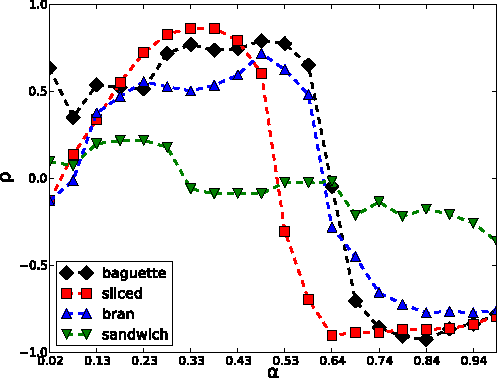
\includegraphics{Fig8}
\caption{\csentence{Spearman correlation coefficients for the FDs and the mean cell area.} (In $[mm^{2}]$, scanned samples).}
\label{fig:corrMCA}
\end{figure*}

\begin{figure*}[h!]
\centering
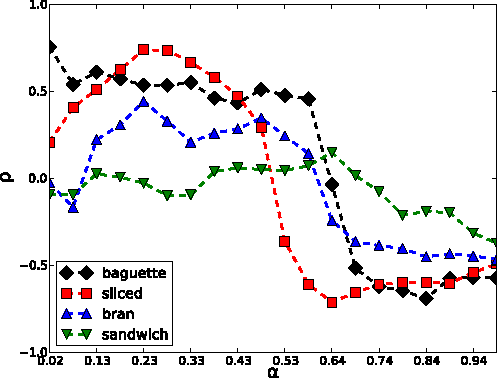
\includegraphics{Fig9}
\caption{\csentence{Spearman correlation coefficients for the FDs and the standard deviation of the mean cell area.} (In $[mm^{2}]$, scanned samples).}
\label{fig:corrMCAstdev}
\end{figure*}



%  \begin{figure}[h!]
%  \caption{\csentence{Sample figure title.}
%      A short description of the figure content
%      should go here.}
%      \end{figure}

%\begin{figure}[h!]
%  \caption{\csentence{Sample figure title.}
%      Figure legend text.}
%      \end{figure}

%%%%%%%%%%%%%%%%%%%%%%%%%%%%%%%%%%%
%%                               %%
%% Tables                        %%
%%                               %%
%%%%%%%%%%%%%%%%%%%%%%%%%%%%%%%%%%%

%% Use of \listoftables is discouraged.
%%
%\section*{Tables}
%\begin{table}[h!]
%\caption{Sample table title. This is where the description of the table should go.}
%      \begin{tabular}{cccc}
%        \hline
%           & B1  &B2   & B3\\ \hline
%        A1 & 0.1 & 0.2 & 0.3\\
%        A2 & ... & ..  & .\\
%        A3 & ..  & .   & .\\ \hline
%      \end{tabular}
%\end{table}

\section*{Tables}
\begin{table}[h!]
% table caption is above the table
\caption{Bread crumb classification results with different number of FDs for the MFS and different classifiers.}
\label{tab:number}       % Give a unique label
% For LaTeX tables use
\begin{tabular}{lllll}
\hline\noalign{\smallskip}
\#FDs & 10  & 20 & 30 \\
\noalign{\smallskip}\hline\noalign{\smallskip}
SVM & \textbf{96\%} & 94.5\% & 95.5\% \\
RF  & 91.5\% & \textbf{93.5\%} & 93\% \\
NN & 88.5\% & \textbf{90.5\%} & 90\% \\
\noalign{\smallskip}\hline
\end{tabular}
\end{table}


\begin{table}[h!]
% table caption is above the table
\caption{Bread crumb classification results using different combinations of the MFS and different classifiers.}
\label{tab:mfs}       % Give a unique label
% For LaTeX tables use
\begin{tabular}{lllll}
\hline\noalign{\smallskip}
Method & MFS & MFS+L & MFS+G & CIELab  \\
\noalign{\smallskip}\hline\noalign{\smallskip}
SVM & 94.5\% & 95.5\% & \textbf{97.5\%} & \textbf{97.5\%} \\
RF  & 93.5\% & \textbf{96\%} & 95\% & \textbf{96\%} \\
NN & 90.5\% & 90\% & 87\% & \textbf{92\%} \\
\noalign{\smallskip}\hline
\#FDs & 20 & 40 & 40 & 60 \\
\hline
\end{tabular}
\end{table}

\begin{table}[h!]
% table caption is above the table
\caption{Bread crumb classification results for different state-of-the-art features and different classifiers.}
\label{tab:other}       % Give a unique label
% For LaTeX tables use
\begin{tabular}{llllll}
\hline\noalign{\smallskip}
Method & Haralick & Lbp & SIFT\\ % & Zernicke
\noalign{\smallskip}\hline\noalign{\smallskip}
SVM & 94\% & 78.5\% & \textbf{96.5\%} \\ % & 55 
RF  & 91\% & 71.5\% & \textbf{92\%} \\ % & 58 
NN & 79\% & 70\% & \textbf{86\%} \\ % & 48.5 
\noalign{\smallskip}\hline
\#FDs & 13 & 36 & 128 \\
\hline
\end{tabular}
\end{table}

\begin{table}[h!]
% table caption is above the table
\caption{Confusion Matrix for the best results (CIELab method, using the SVM classifier).}
\label{tab:confusionmatrix}       % Give a unique label
% For LaTeX tables use
\begin{tabular}{llllll}
\hline\noalign{\smallskip}
Class&{\em baguette} & {\em sliced} & {\em bran} &{\em sandwich}&{\em nonbread} \\
\noalign{\smallskip}\hline\noalign{\smallskip}
{\em baguette} & 39& 1 &1 &0 &0 \\
{\em sliced} & 0& 38 &0 &0 &0  \\
{\em bran} & 0& 0 &39 &1 &0  \\
{\em sandwich} & 1& 1 &0 &39 &0  \\
{\em nonbread} & 0& 0 &0 &0 &40  \\
\hline
\end{tabular}
\end{table}

%%%%%%%%%%%%%%%%%%%%%%%%%%%%%%%%%%%
%%                               %%
%% Additional Files              %%
%%                               %%
%%%%%%%%%%%%%%%%%%%%%%%%%%%%%%%%%%%

%\section*{Additional Files}
%  \subsection*{Additional file 1 --- Sample additional file title}
%    Additional file descriptions text (including details of how to
%    view the file, if it is in a non-standard format or the file extension).  This might
%    refer to a multi-page table or a figure.

%  \subsection*{Additional file 2 --- Sample additional file title}
%    Additional file descriptions text.



\end{backmatter}
\end{document}
